\documentclass[12pt,a4paper]{article}
%\usepackage[UTF8]{ctex}
\usepackage{amsfonts,amsmath,amsthm,amssymb}
\usepackage{mathtools}
\usepackage{sfmath}
\usepackage{hyperref}
\renewcommand{\familydefault}{\sfdefault}
\usepackage{geometry}
\geometry{left=0cm,right=0cm,top=0cm,bottom=0.1cm, footskip=0cm, includefoot=true}
\pagestyle{empty}
\setcounter{secnumdepth}{4}

\usepackage[all]{xy}
\usepackage{color}
\usepackage{tikz}
\usetikzlibrary{arrows.meta}
\usetikzlibrary{calc}

\usepackage{titlesec}
\titleformat{\section}[block]{\huge\bfseries\sffamily}{\thesection}{1em}{}
\titleformat{\subsection}[block]{\huge\bfseries\sffamily}{\thesubsection}{1em}{}
\titleformat{\subsubsection}[block]{\huge\bfseries\sffamily}{\thesubsubsection}{1em}{}
\titleformat{\paragraph}[block]{\huge\bfseries\sffamily}{\theparagraph}{1em}{}
\titlespacing*{\paragraph}{0pt}{1ex}{0.5ex}

\renewenvironment{proof}{{\noindent\it\textbf{Proof}}\quad\it}{\hfill$\square$}

%\theoremstyle{definition}

\newtheorem{thm}[equation]{Theorem}
\newtheorem{cor}[equation]{Corollary}
\newtheorem{lem}[equation]{Lemma}
\newtheorem{prop}[equation]{Proposition}
\newtheorem{defn}[equation]{Definition}
\newtheorem{rem}[equation]{Remark}
\newtheorem{conj}[equation]{Conjecture}
\newtheorem{notation}[equation]{Notation}
\newtheorem{definition}[equation]{Definition}
\newtheorem{remark}[equation]{Remark}
\newtheorem{example}[equation]{Example}
\newtheorem{proposition}[equation]{Proposition}
\newtheorem{theorem}[equation]{Theorem}
\newtheorem{lemma}[equation]{Lemma}
\newtheorem{corollary}[equation]{Corollary}

\newcommand{\Z}{\mathbb{Z}}
\newcommand{\Ext}{\operatorname{Ext}}

\newcommand{\AF}{\mathrm{AF}}
\newcommand{\ESS}[1]{\prescript{#1\!}{}{E}}
\newcommand{\ZESS}[1]{\prescript{#1\!}{}{Z}}
\newcommand{\BESS}[1]{\prescript{#1\!}{}{B}}
\newcommand{\SynSS}{\prescript{\mathrm{syn}\!}{}{E}}
\newcommand{\HF}{\mathrm{H}\mathbb{F}_2}
\newcommand{\Sus}{\Sigma}
\newcommand{\iso}{\cong}
\newcommand{\calSyn}{\mathcal{S}\mathrm{yn}}
\newcommand{\calSp}{\mathcal{S}\mathrm{p}}
\newcommand{\fto}[1]{\xrightarrow{#1}}
\newcommand{\sma}{\wedge}

% Define tikz colors
\definecolor{lightgray}{RGB}{200,200,200}
\definecolor{llgray}{RGB}{235,235,235}

% draw grid in tikz
% params: x1,x2,y1,y2
\newcommand{\tikzgrid}[4]{\foreach \x in {#1,...,#2} {
        \draw[black!20] (\x-0.5, #3-0.5) -- (\x-0.5, #4-0.5);
    }
    \foreach \y in {#3,...,#4} {
        \draw[black!20] (#1-0.5, \y-0.5) -- (#2-0.5, \y-0.5);
    }
}

\newcommand{\drawarrow}{\draw[-{Stealth[length=1.5mm]}, shorten >=(0.08cm)]}

\title{The Generalized Leibniz Rule and Generalized Mahowald Trick}
\author{}


\begin{document}

\sffamily
\maketitle
\thispagestyle{empty}

\huge

\begin{sloppy}
\clubpenalty=-100
\widowpenalty=-100

\section{The Generalized Leibniz Rule and Generalized Mahowald Trick} \label{sec:rules}

\section{generalization Leibnitz rule}
Now, we introduce the theorem of the Generalized Leibniz Rule, a valuable tool for computing new Adams differentials.

\begin{theorem}[Generalized Leibniz Rule]\label{thm:e73f481e}
    Let $f: X\to Y$ be a map between two classical spectra.
    Suppose that $2\le n\le r$, $e(f)\le m\le n-2+e(f)$, $l\ge e(f)$, and we have
    $$x\in Z_{r-1}^{s,t}(X), \hspace{0.5cm} y\in Z_{r-1-m+e(f)}^{s+m,t+m}(Y)$$
    $$x_\infty\in Z_\infty^{s+r,t+r-1}(X), \hspace{0.5cm} y_\infty\in Z_\infty^{s+r+l,t+r+l-1}(Y)$$
    and the following conditions hold:
    \begin{enumerate}
        \item $d_{r}(x)=x_\infty$,
        \item $d_{m}^{f,E_n}(x)=y$,
        \item $d_{l}^{f,E_\infty}(x_\infty)=y_\infty$,
        \item the differential in (1) has no crossing on the $E_n$-page or (2) has no crossing.
        \item the differential in (3) has no crossing.% on the $E_\infty$-page.
    \end{enumerate}
    Then we have an Adams differential
    $$d_{r+l-m}(y)= y_\infty.$$
\end{theorem}

\begin{proof}
    Consider the commutative diagram of synthetic spectra
    $$\xymatrix{
        \Sus^{0,e(f)}\nu X/\lambda^{n-1} \ar[rr]^{\hat f_{n-1}}\ar[d]_{\delta_X} && \nu Y/\lambda^{n-1}\ar[d]_{\delta_Y}\\
        \Sus^{1,-n+1+e(f)} \nu X \ar[rr]_{\hat f} && \Sus^{1,-n+1}\nu Y.
    }$$
    By condition (1) and Proposition \ref{prop:6de7d130}, we have
    \begin{equation}\label{eq:ca3fdd92}
        d^{\delta_X}_r(x)=\lambda^{r-n}x_\infty.
    \end{equation}
    By conditions (2) and (3), and Definition \ref{def:6c076a33}, we have
    \begin{equation}\label{eq:b2aa5032}
        d^{\hat f_{n-1}}_m(x)=\lambda^{m-e(f)} y
    \end{equation}
    and
    \begin{equation*}
        d^{\hat f}_l(x_\infty)=\lambda^{l-e(f)} y_\infty,
    \end{equation*}
    which implies
    \begin{equation}\label{eq:886aee9b}
         d^{\hat f}_l(\lambda^{r-n}x_\infty)=\lambda^{r+l-n-e(f)}y_\infty.
    \end{equation}

    Applying Proposition \ref{prop:cross-dr-En} and Proposition \ref{prop:cross-f-Er} to conditions (4) and (5), we know that the differential in (\ref{eq:ca3fdd92}) or (\ref{eq:b2aa5032}) has no crossing, and that the differential in (\ref{eq:886aee9b}) has no crossing.

    Therefore, we can apply Corollary \ref{cor:0012nik} and obtain
    $$d^{\delta_Y}_{r+l-m}(\lambda^{m-e(f)} y)=\lambda^{r+l-n-e(f)} y_\infty.$$
    By Remark \ref{rmk:qvoewfj}, this is equivalent to
    $$d_{r+l-m}(y)= y_\infty.$$
\end{proof}

\begin{theorem}[Generalized Leibniz Rule]\label{thm:e73f481eB}
    Let $f: X\to Y$ be a map between two classical spectra.
    Suppose that $2\le n\le r$, $e(f)\le m\le n-2+e(f)$, $l\ge e(f)$, and we have
    $$x\in Z_{r-1}^{s,t}(X), \hspace{0.5cm} y\in Z_{r-1-m+e(f)}^{s+m,t+m}(Y)$$
    $$x_\infty\in Z_\infty^{s+r,t+r-1}(X), \hspace{0.5cm} y_\infty\in Z_\infty^{s+r+l,t+r+l-1}(Y)$$
    and the following conditions hold:
    \begin{enumerate}
        \item $d_{r}(x)=x_\infty$,
        \item $d_{m}^{f,E_n, k}(x)=y$,
        \item $d_{l}^{f,E_\infty, k}(x_\infty)=y_\infty$,
        \item the differential in (1) has no crossing on the $E_n$-page or (2) has no crossing.
        \item the differential in (3) has no crossing.% on the $E_\infty$-page.
    \end{enumerate}
    Then we have an Adams differential
    $$d_{r+l-m}(y)= y_\infty.$$
\end{theorem}

\begin{proof}
    Consider the commutative diagram of synthetic spectra
    $$\xymatrix{
        \Sus^{0,e(f)}\nu X/\lambda^{n-1} \ar[rr]^{\hat f_{n-1}}\ar[d]_{\delta_X} && \nu Y/\lambda^{n-1}\ar[d]_{\delta_Y}\\
        \Sus^{1,-n+1+e(f)} \nu X \ar[rr]_{\hat f} && \Sus^{1,-n+1}\nu Y.
    }$$
    By condition (1) and Proposition \ref{prop:6de7d130}, we have
    \begin{equation}\label{eq:ca3fdd92B}
        d^{\delta_X}_r(x)=\lambda^{r-n}x_\infty.
    \end{equation}
    By conditions (2) and (3), and Definition \ref{def:6c076a33}, we have
    \begin{equation}\label{eq:b2aa5032B}
        d^{\hat f_{n-1}}_m(\lambda^k x)=\lambda^{m-e(f)+k} y
    \end{equation}
    and
    \begin{equation*}
        d^{\hat f}_l(\lambda^k x_\infty)=\lambda^{l-e(f)+k} y_\infty,
    \end{equation*}
    which implies
    \begin{equation}\label{eq:886aee9bB}
         d^{\hat f}_l(\lambda^{r-n+k}x_\infty)=\lambda^{r+l-n-e(f)+k}y_\infty.
    \end{equation}

    Applying Proposition \ref{prop:cross-dr-En} and Proposition \ref{prop:cross-f-Er} to conditions (4) and (5), we know that the differential in (\ref{eq:ca3fdd92B}) or (\ref{eq:b2aa5032B}) has no crossing, and that the differential in (\ref{eq:886aee9bB}) has no crossing.

    Therefore, we can apply Corollary \ref{cor:0012nik} and obtain
    $$d^{\delta_Y}_{r+l-m}(\lambda^{m-e(f)+k} y)=\lambda^{r+l-n-e(f)+k} y_\infty.$$
    By Remark \ref{rmk:qvoewfj}, this is equivalent to
    $$d_{r+l-m}(y)= y_\infty.$$
\end{proof}

\begin{remark}
    We can further generalize Theorem \ref{thm:e73f481e} by using the conditions in Theorem \ref{thm:4114f70c} rather than those Corollary \ref{cor:0012nik}. We leave this generalization to the reader.

    try to do this.
\end{remark}

We emphasize that the no-crossing conditions in Theorem \ref{thm:e73f481e}, the Generalized Leibniz Rule, are crucial. We first demonstrate the strength of the Generalized Leibniz Rule with Example~\ref{exam:Leibnizyes}, which uses a $d_2$-differential to prove a $d_3$-differential in the classical Adams spectral sequence. Additionally, Example~\ref{exam:Leibnizno} shows that, without the no-crossing condition, the conclusion could be false.

\subsection{Generalized Mahowald trick}
Next, we discuss the Generalized Mahowald Trick.

In order to apply the Generalized Leibniz Rule, we need to provide a method for computing extensions on specific Adams $E_k$-pages, such as the $(f, E_3)$-extension $d_2^{f, E_3} (h_0h_4^2) = h_0 p$ in Example~\ref{exam:Leibnizyes}. This is provided by Theorem~\ref{thm:158d451a} (the Generalized Mahowald Trick). The crux of the proof of the Generalized Mahowald Trick lies in the following lemma.
\begin{lemma}[May \cite{May01}]\label{lem:452d218c}
    Let $X\to Y\to Z\to \Sus X$ and $X'\to Y'\to Z'\to \Sus X'$ be distinguished triangles of (synthetic) spectra. By smashing these distinguished triangles together, we obtain the following commutative diagram of cofiber sequences:
    $$\xymatrix{
    X\sma X' \ar[r] \ar[d] & Y\sma X' \ar[r] \ar[d] & Z\sma X' \ar[d]\\
    X\sma Y' \ar[d] \ar[r] & Y\sma Y' \ar[d] \ar[r] & Z\sma Y' \ar[d]\\
    X\sma Z' \ar[r] & Y\sma Z' \ar[r] & Z\sma Z'\\
    }$$
    If $a\in \pi_n(X\sma Z')$ and $b\in\pi_n(Y\sma Y')$ map to the same element in $\pi_n(Y\sma Z')$, then there exists $c\in \pi_n(Z\sma X')$ such that
    \begin{enumerate}
        \item $b$ and $c$ map to the same element in $\pi_n(Z\sma Y')$, and
        \item $a$ and $c$ map to the same element via boundary maps in $\pi_{n-1}(X\sma X')$.
    \end{enumerate}
\end{lemma}

\begin{proof}
The proof follows directly from \cite[Lemma 4.6]{May01}.

In fact, consider $V$ in Axiom TC3 of \cite[Section 4]{May01} and the corresponding commutative diagram. By \cite[Lemma 4.6]{May01} we know that $V$ is the pull back of the following diagram.
$$\xymatrix{
\ar@{}[dr]|\lrcorner V\ar[d]\ar[r]& Y\sma Y'\ar[d]\\
X\sma Z'\ar[r] & Y\sma Z'
}$$
Since $a$ and $b$ map to the same element in $\pi_n(Y\sma Z')$, we know that we can find $v\in V$ such that $v$ maps to $a$ in $\pi_n(X\sma Z')$ and $b$ in $\pi_n(Y\sma Y')$. Then we let $c=j_3(v)\in \pi_n(Z\sma X')$, where $j_3: V \rightarrow Z \sma X'$ is the map in the commutative diagram in Axiom TC3 of \cite[Section 4]{May01}. This lemma follows from the commutativity of the diagram.
\end{proof}

\begin{theorem}[Generalized Mahowald Trick]\label{thm:158d451a}
    Consider a distinguished triangle of spectra
    $$X\fto{f} Y\fto{g} Z\fto{h} \Sus X$$
    with $e(f)+e(g)+e(h)=1$.
    Suppose that $r=n+m+l$, $n_1=n-e(f)\ge 1$, $m_1=m-e(g)\ge 0$, $l_1=l-e(h)\ge 0$, and
    $$\begin{array}{ll}
        x\in Z_{n_1}^{s+l,t+l-1}(X), & y\in Z_{m_1+1}^{s+n+l,t+n+l-1}(Y),\\
        \bar x\in Z_{r-1}^{s,t}(Z), & \bar y\in Z_\infty^{s+r,t+r-1}(Z),
    \end{array}$$
    such that
    \begin{enumerate}
        \item $d^{h,E_{r'}}_{l}\bar x=x$, where $r'=r-m_1=n_1+l_1+1$,
        \item $d_r \bar x=\bar y$,
            \item the $(h,E_{r'})$-extension in (1) has no crossing, or the Adams differential (2) has no crossing on the $E_{r'}$-page,
        \item $d^{g,E_{m_1+2}}_{m}y=\bar y$.
    \end{enumerate}
    Then we have $x\in Z_{n+m+e(h)}^{s+l,t+l-1}(X)$ and
    $$d^{f,E_{n+m+1+e(h)},l_1}_{n}x\equiv y \mod %B_{r'}^{s+n+l,t+n+l-1}(Y).
    \text{someting}$$
    (See Figure \ref{fig:2aa45b21}.)
\end{theorem}
\begin{figure}[h]
\centering
\scalebox{0.9}{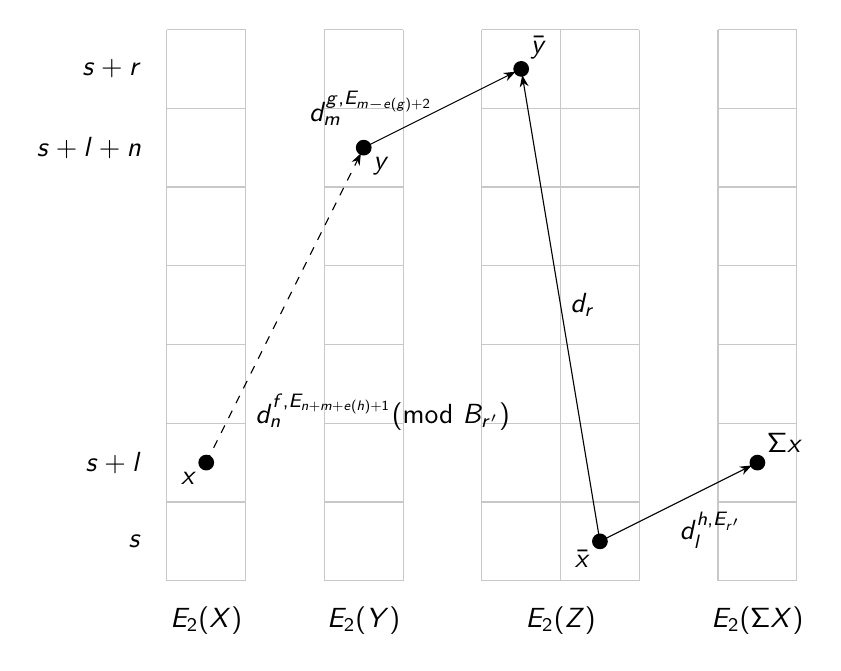
\begin{tikzpicture}[node/.style={circle,fill=black!0.1}]
    \def\ymax{6}
    \def\ymaxp{7}

    % Draw grid
    \foreach \x in {0,...,8} {
        \draw[lightgray] (\x-0.5, -0.5) -- (\x-0.5, \ymax+0.5);
    }
    \foreach \x in {0,2,4,5,7} {
        \foreach \y in {0,...,\ymaxp} {
            \draw[lightgray] (\x-0.5, \y-0.5) -- (\x+0.5, \y-0.5);
        }
    }

    % Draw bullets
    \coordinate (x) at (0, 1);
    \coordinate (y) at (2, 5);
    \coordinate (y1) at (4, 6);
    \coordinate (x1) at (5, 0);
    \coordinate (sx) at (7, 1);

    \fill (x) circle (0.1) node[below left] {$x$};
    \fill (y) circle (0.1) node[below right] {$y$};
    \fill (x1) circle (0.1) node[below left] {$\bar x$};
    \fill (y1) circle (0.1) node[above right] {$\bar y$};
    \fill (sx) circle (0.1) node[above right] {$\Sus x$};

    % Draw differentials
    \draw[dashed, -{Stealth[length=1.5mm]}, shorten >=(0.08cm)] (x) -- (y) node[near start,below right] {$d^{f, E_{n+m+e(h)+1}}_n(\mathrm{mod}~B_{r'})$};
    \drawarrow (y) -- (y1) node[midway,left] {$d^{g,E_{m-e(g)+2}}_{m}$};
    \drawarrow (x1) -- (y1) node[midway,right] {$d_r$};
    \drawarrow (x1) -- (sx) node[midway,below] {~\hspace{2em}$d^{h,E_{r'}}_{l}$};

    \node[anchor=east] at (-.7, 0) {$s$};
    \node[anchor=east] at (-.7, 1) {$s+l$};
    \node[anchor=east] at (-.7, 5) {$s+l+n$};
    \node[anchor=east] at (-.7, 6) {$s+r$};

    \node at (0, -1.0) {$E_2(X)$};
    \node at (2, -1.0) {$E_2(Y)$};
    \node at (4.5, -1.0) {$E_2(Z)$};
    \node at (7, -1.0) {$E_2(\Sus X)$};
\end{tikzpicture}}
\caption{A demonstration of Theorem \ref{thm:158d451a}}\label{fig:2aa45b21}
\end{figure}

\begin{figure}
\centering
    \scalebox{0.85}{$\xymatrix@C=1em{
        \bigwedge & \nu X \ar[r]^-{\hat f} & \Sus^{0,-\!e(f)}\nu Y \ar[r]^-{\hat g} &  \Sus^{0,-\!e(f)\!-\!e(g)}\nu Z \ar[r]^-{\hat h} & \Sus^{1,0}\nu X\\
        S^{0,0}/\lambda^{r} \ar[d]_{\rho} & & & & [\lambda^{l_1}x] \ar[d]\\
        S^{0,0}/\lambda^{r'-1} \ar[d]_{\delta_{r'-1}} & & & [\bar x] \ar[r] \ar[d] & [\lambda^{l_1}x]\\
        S^{1,-r'+1}/\lambda^{m_1+1} \ar[d]_{\lambda^{r'-1}} & & [y] \ar[r] \ar[d] & [\lambda^{m_1}\bar y] & \\
        S^{1,0}/\lambda^{r} & [\lambda^{l_1}x] \ar[r] & [\lambda^{r'-1}y] & & \\
    }$}
\caption{Elements in the homotopy groups of the smash products}\label{fig:2d013742}
\end{figure}

\begin{proof}
    Consider the following two distinguished triangles of synthetic spectra
    \begin{gather*}
        \nu X\fto{\hat f} \Sus^{0,-e(f)}\nu Y\fto{\hat g} \Sus^{0,-e(f)-e(g)}\nu Z\fto{\hat h} \Sus^{0,-1}\nu \Sus X=\Sus^{1,0}\nu X\\
        S^{0,0}/\lambda^{r}\fto{\rho} S^{0,0}/\lambda^{r'-1} \fto{\delta_{r'-1}} S^{1,-r'+1}/\lambda^{m_1+1} \fto{\lambda^{r'-1}} S^{1,0}/\lambda^{r}
    \end{gather*}
    and their smash product. See Figure \ref{fig:2d013742}.

    By condition (1), we have
    \begin{equation}\label{eq:70327019}
        d^{\hat h_{r'-1}}_l(\bar x)=\lambda^{l_1}x
    \end{equation}
    where $\hat h_{r'-1}$ is the map $\Sus^{0,e(h)}\nu Z/\lambda^{r'-1}\to \nu X/\lambda^{r'-1}$ induced by $\hat h$.
    By condition (2), we have
    \begin{equation}\label{eq:e129d90c}
        d^{\delta_{r'-1}}_r(\bar x)=\lambda^{m_1}\bar y.
    \end{equation}


    Applying Proposition \ref{prop:cross-dr-En} and Proposition \ref{prop:cross-f-Er} to condition (3), we know that the differential in (\ref{eq:70327019}) or the differential in (\ref{eq:e129d90c}) has no crossing. Hence, there exists
    $$[\bar x]\in \{\bar x\}\subset \pi_{t-s,t}(\nu Z/\lambda^{r'-1})$$
    such that
    $$\hat h_{r'-1}([\bar x])\in \{\lambda^{l_1}x\}\subset \pi_{t-s-1, t-1+e(h)}(\nu X/\lambda^{r'-1})$$
    and
    $$\delta_{r'-1}([\bar x])\in \{\lambda^{m_1}\bar y\}\subset \pi_{t-s-1,t+r'-1}(\nu Z/\lambda^{m_1+1}).$$

    By condition (4), we have
    \begin{equation*}
        d^{\hat g_{m_1+1}}_m(y)=\lambda^{m_1}\bar y.
    \end{equation*}
    This implies that there exists
    $$[y]\in \{y\}\subset \pi_{t-s-1,t+n+l-1}(\nu Y/\lambda^{m_1+1})$$
    such that
    $$\hat g_{m_1+1}([y])\in \{\lambda^{m_1}\bar y\}\subset \pi_{t-s-1, t+r'-1}(\nu Z/\lambda^{m_1+1}),$$
    where $\hat g_{m_1+1}$ is the map $\Sus^{0,e(g)}\nu Y/\lambda^{m_1+1}\to \nu Z/\lambda^{m_1+1}$ induced by $\hat g$.

    Due to degree reasons (Proposition \ref{prop:59f111f}), $\lambda^{m_1}\bar y$ detects a unique element in homotopy,
    $$[\lambda^{m_1}\bar y]\in \pi_{t-s-1, t+r'-1}(\nu Z)/\lambda^{m_1+1}.$$
    Therefore, we have
    $$\delta_{r'-1}([\bar x])=\hat g_{m_1+1}([y])=[\lambda^{m_1}\bar y],$$
    By Lemma \ref{lem:452d218c}, there exists
    $$[\lambda^{l_1}x]\in \pi_{t-s-1,t-1+e(h)}(\nu X/\lambda^r),$$
    such that
    \begin{gather}
        \rho ([\lambda^{l_1}x])=\hat h_{r'-1}([\bar x]),\label{eq:f4848f29}\\
        \hat f_r([\lambda^{l_1}x])=\lambda^{r'-1}[y],\label{eq:fba35e4e}
    \end{gather}
    where $\rho$ is the map $\nu X/\lambda^r\to \nu X/\lambda^{r'-1}$, and $\hat f_r$ is the map $\Sus^{0,e(f)}\nu X/\lambda^r\to \nu Y/\lambda^r$ induced by $\hat f$.

    The equality in (\ref{eq:f4848f29}) indicates that $[\lambda^{l_1}x]$ can be lifted to the $E_\infty$-page of $\nu X/\lambda^r$, so we have
    $$x\in Z_{n+m+e(h)}^{s+l,t+l-1}(X).$$
    The equation in (\ref{eq:fba35e4e}) indicates that
    $$d^{\hat f_r}_n(\lambda^{l_1}x)=\lambda^{r'-1}y.$$
    %Therefore, by dividing $\lambda^{l_1}$, we have
    %$$d^{\hat f_{n+m+e(h)}}_n(x)\equiv \lambda^{n_1}y \mod B_{r'}^{s+n+l,t+n+l-1}(Y)$$
    %for $x$ in the $E_\infty$ page of $\nu X/\lambda^{r-l_1}=\nu X/\lambda^{n+m+e(h)}$.
     By definition, this is equivalent to
    $$d^{f, E_{n+m+1+e(h)}, l_1}_nx\equiv y \mod %B_{r'}^{s+n+l,t+n+l-1}(Y).
    \text{someting}$$
\end{proof}

\paragraph{}
There is also a version of the generalized Mahowald trick where the assumtion is g and h extensions at level $k$, try to do this generalization.

\subsection{Extensions in different pages}
    We refer to Theorem~\ref{thm:158d451a} as the Generalized Mahowald Trick, as this approach was first utilized by Mahowald and his collaborators in various works (see, for example, \cite{MahowaldTangora}), particularly in the case where $m_1 = l_1 = 0$. The synthetic setting advances this method by allowing for the consideration of cases where $m_1>0, l_1>0$ as well.
The outcome of the Generalized Mahowald Trick, as stated in Theorem~\ref{thm:158d451a}, is an $f$-extension on a specific Adams page, such as the $(f, E_3)$-extension $d_2^{f, E_3} (h_0h_4^2) = h_0 p$ in Example~\ref{exam:extonEn}(2) and Example~\ref{exam:Mahowald}. In practice, the source of an $(f, E_r)$-extension may survive to later Adams pages, prompting interest in the $(f, E_{>r})$-extensions, such as the $(f, E_\infty)$-extension $d_2^{f, E_\infty} (h_0h_4^2) = h_0 p$ in Example~\ref{exam:extonEn}(3), which is applied in Example~\ref{exam:Leibnizyes}. The following Propositions~\ref{prop:dec738d3} and \ref{cor:dfc6043e} describe the relationships between extensions across different pages.

\begin{proposition}\label{prop:dec738d3}
    Suppose that we have an $(f,E_r)$-extension $d^{f,E_r}_n(x)=y$, where $x\in Z_{r-1}^{s,t}(X)$ and $y\in Z_{r-1-n+e(f)}^{s+n,t+n}(Y)$. Then for all $2\le r'<r$, we also have
    \begin{equation}\label{eq:dr'}
        d^{f,E_{r'}}_n(x)=y.
    \end{equation}

    Furthermore, if $d^{f,E_r}_n(x)=y$ is essential and $n\le r'-2+e(f)$, then (\ref{eq:dr'}) is inessential if and only if there exists some $0<a'\le n-e(f)$ and an element
    $$x'\in Z_{r'-1-a'}^{s+a',t+a'}(X)\backslash Z_{r-1-a'}^{s+a',t+a'}(X)$$
    such that
    $$d^{\hat f_{r'-1}}_{n-a'-b}(\lambda^{a'} x')=\lambda^{n-b-e(f)} y'$$
    for some $b\ge 0$.

\end{proposition}

\begin{proof}
    Consider the following commutative diagram:
    $$\xymatrix{
        \Sus^{0,e(f)}\nu X/\lambda^{r-1} \ar[r]^-{\hat f_{r-1}}\ar[d]_{\rho_X} & \nu Y/\lambda^{r-1} \ar[d]_{\rho_Y}\\
        \Sus^{0,e(f)}\nu X/\lambda^{r'-1} \ar[r]^-{\hat f_{r'-1}} & \nu Y/\lambda^{r'-1}
    }$$
    By Corollary \ref{cor:e7b20ae2}, $(\rho_X,\rho_Y)$ induces a map from the $\hat f_{r-1}$-ESS to the $\hat f_{r'-1}$-ESS. Therefore, by naturality,
    $$d^{\hat f_{r-1}}_n(x)=\lambda^{n-e(f)} y\ \text{implies} \ d^{\hat f_{r'-1}}_n(x)=\lambda^{n-e(f)} y,$$
    which, by definition, is
    $$d^{f,E_{r'}}_n(x)=y.$$

    Next, we prove the second part of the proposition. By Definition \ref{def:6c076a33}, the $(f,E_r)$-extension (\ref{eq:dr'}) is inessential if and only if
    there exists $0<a\le n-e(f)$ and
    $$\lambda^a x'\in E_\infty^{s+a,t+a,t}(\nu X/\lambda^{r'-1})\iso Z_{r'-1-a}^{s+a,t+a}(X)/B_{1+a}^{s+a,t+a}(X),$$
    such that
    \begin{equation}\label{eq:dcd62a19}
        d^{\hat f_{r'-1}}_{n-a}(\lambda^ax')=\lambda^{n-e(f)} y,
    \end{equation}
    and this differential is not induced by $(\rho_X,\rho_Y)$, as we assume that $d^{f,E_r}_n(x)=y$ is essential.

    There are two scenarios where this differential is not induced by $(\rho_X,\rho_Y)$. The first case occurs when $\lambda^ax'$ is not in the image of $\rho_X$ at all, which is equivalent to $x'\notin Z_{r-1-a}^{s+a,t+a}(X)$. (See Figure \ref{fig:b22d961f}.)

    \begin{figure}[h]
    \centering
    \scalebox{0.9}{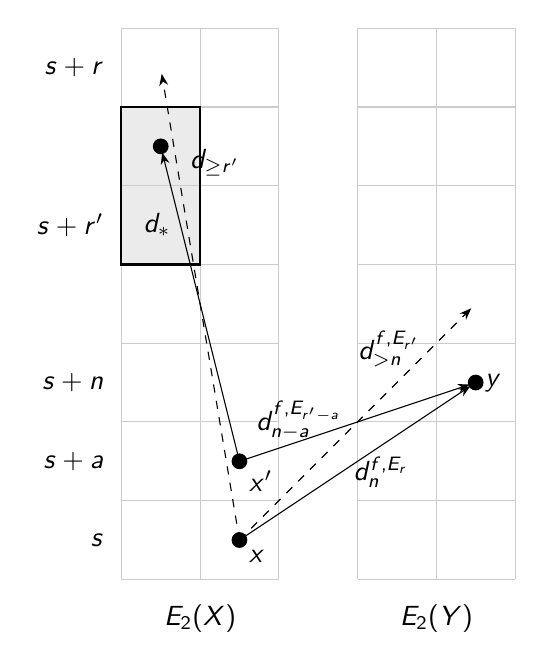
\begin{tikzpicture}
        % Draw grid
        \fill[llgray] (0-0.5, 4-0.5) rectangle ++(1, 2);
        \tikzgrid{0}{2}{0}{7}
        \tikzgrid{3}{5}{0}{7}
        \draw[thick] (0-0.5, 4-0.5) rectangle ++(1, 2);

        % Draw bullets
        \coordinate (x) at (1, 0);
        \coordinate (x1) at (1, 1);
        \coordinate (dx1) at (0, 5);
        \coordinate (dx) at (0, 6);
        \coordinate (y) at (4, 3);
        \coordinate (y1) at (4, 2);
        \coordinate (dy) at (3, 6);

        \fill (x) circle (0.1) node[below right] {$x$};
        \fill (x1) circle (0.1) node[below right] {$x'$};
        \fill (y1) circle (0.1) node[right] {$y$};
        \fill (dx1) circle (0.1) node[right] {};

        % Draw differentials
        \draw[dashed, -{Stealth[length=1.5mm]}, shorten >=(0.08cm)] (x) -- (dx) node[near end, above right] {$d_{\ge r'}$};
        \drawarrow (x1) -- (dx1) node[near end,left] {$d_*$};
        \draw[dashed, -{Stealth[length=1.5mm]}, shorten >=(0.08cm)] (x) -- (y) node[near end,above left=-5pt] {$d^{f,E_{r'}}_{>n}$};
        \drawarrow (x) -- (y1) node[midway,below right=-5pt] {$d^{f,E_{r}}_{n}$};
        \drawarrow (x1) -- (y1) node[near start,above=-3pt] {$d^{f,E_{r'-a}}_{n-a}$};

        \node[anchor=east] at (-0.6, 0) {$s$};
        \node[anchor=east] at (-0.6, 1) {$s+a$};
        \node[anchor=east] at (-0.6, 2) {$s+n$};
        \node[anchor=east] at (-0.6, 4) {$s+r'$};
        \node[anchor=east] at (-0.6, 6) {$s+r$};

        \node at (.5, -1.0) {$E_2(X)$};
        \node at (3.5, -1.0) {$E_2(Y)$};
    \end{tikzpicture}}
    \caption{Extensions across pages}\label{fig:b22d961f}
    \end{figure}

    The second case occurs when $\lambda^ax'$ is in the image of $\rho_X$, but it supports an essential $\hat f_{r-1}$-extension that is strictly shorter than the differential (\ref{eq:dcd62a19}).

    To further explore this scenario, we replace $x$ with $\lambda^ax'$ and analyze successive essential extensions. This process is repeated iteratively until the first case is reached. Ultimately, this leads to the existence of some $0<a'\le n-e(f)$ and an element
    $$x''\in Z_{r'-1-a'}^{s+a',t+a'}(X)\backslash Z_{r-1-a'}^{s+a',t+a'}(X)$$
    such that
    $$d^{\hat f_{r'-1}}_{n-a'-b}(\lambda^{a'} x'')=\lambda^{n-b-e(f)} y'$$
    for some $b>0$. This represents a crossing of $d^{\hat f_{r'-1}}_n(x)=\lambda^{n-e(f)}y$.

\end{proof}


The following Corollary~\ref{cor:dfc6043e} is the contrapositive statement of the second part of Proposition~\ref{prop:dec738d3}.


\begin{corollary}\label{cor:dfc6043e}
    Suppose $r\ge r'$ and there exists an $(f,E_{r'})$-extension
    $$d^{f,E_{r'}}_n(x)=y$$
    for $x\in Z_{r-1}^{s,t}(X)$ and $y\in Z_{r'-1-n+e(f)}^{s+n,t+n}(Y)$. Assume that this extension has no crossing of the form $d^{f,E_{r'-a}}_{n-a-b}(x')=y'$ for any $b>0$, $0<a\le n-e(f)$, and
    $$x'\in Z_{r'-1-a}^{s+a,t+a}(X)\backslash Z_{r-1-a}^{s+a,t+a}(X).$$
    Under these conditions, we also have an $(f,E_{r})$-extension
    $$d^{f,E_{r}}_n(x)=y.$$
\end{corollary}


\begin{example} \label{exam:stretchext}
    In Example~\ref{exam:Mahowald}, we use the Generalized Mahowald Trick to establish the $(f, E_3)$-extension:
        $$d_2^{f, E_3} (h_0h_4^2) = h_0 p,$$
        for the map $f=\nu:S^3 \rightarrow S^0$, as discussed
in Example~\ref{exam:extonEn}(2). However, to apply the Generalized Leibniz Rule in proving the classical Adams differential
$$d_3(h_2h_5) = h_0p$$
in Example~\ref{exam:Leibnizyes}, we need the $E_\infty$-page version of the $(f, E_3)$-extension:
$$d_2^{f, E_\infty} (h_0h_4^2) = h_0 p.$$
We apply Corollary~\ref{cor:dfc6043e} to confirm this.

As checked in Example~\ref{exam:Ercross}(2), the $(f, E_3)$-extension has no crossing. Consequently, by Corollary~\ref{cor:dfc6043e}, we obtain the required $(f, E_\infty)$-extension:
$$d_2^{f, E_\infty} (h_0h_4^2) = h_0 p.$$
\end{example}

\end{sloppy}
\end{document}
